\newpage
\section{Umsetzung der Positionsbestimmung}

Nachdem die theroretische Einleitung abgeschlossen ist, widmen wir uns in diesem Kapitel der konkreten Umsetzung der Positionsbestimmung.

\subsection{Hardwareimplementierung}
Es wird die Position von dem Master bestimmt. Die Slaves sitzen dabei an bekannten XY-Koordinaten. Weitherhin besitzt der Master das \microphone \platz Mikrofon, weil es günstiger ist, als jeden Slave mit einem  Mikrofon auszustatten. Die Accesspoints besitzen dementsprechend ein Lautsprecher. Die folgende Abbildung \ref{img:blockschaltbild} ist ein Blockschaltbild, welches die Hardware von dem Zielknoten und dem Accesspoint zeigt. Accesspoint und Zielknoten kommunizieren über das \SI{2,4}{GHz} Band drahtlos miteinander.

\begin{figure}[H]
        \centering
        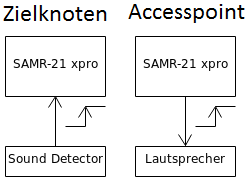
\includegraphics[width=0.5\textwidth]{images/blockschaltbild.png}
        \caption{Aufbau des Zielknoten und Accesspoint}
        \label{img:blockschaltbild}
\end{figure}

\subsection{Softwareimplementierung}

\subsubsection{Kommunikation Zielknoten -- Accesspoint}\mbox{}\\
Für die Kommunikation zwischen Zielknoten und Accespoint wird die Frequenz $2,4 \;GHz$ verwendet. Die Kommunikation teilt sich in Master und Slave auf. Der Master ist der Zielknoten. Die Accesspoint die Slaves. Die Slaves dürfen nur antworten, wenn zuvor vom Master eine Anfrage kam.
\\
Für die Kommunikation wird das UDP - Protokoll verwendet. Dabei ist die Portnummer die eindeutige Kennung jeden Slaves. Slaves nehmen nur Pakete entgegen, wenn die Portnummer mit ihrer Kennung übereinstimmt. Die Kommunikation erfolgt über ein definiertes Datenstruktur. Die Datenstruktur beinhaltet folgende Variablen.
\newpage
\begin{description}[style=multiline,leftmargin=3cm]
\item [port] 	Port des Zielrechners
\item [cmd]  	Steuercode
\item [systime]	Aktuelle Systemzeit des Senders
\item [data]	Payload
\item [array {[5]}]	Weiterer Payload
\item [len\_ array]	Länge des Array
\end{description}

Steuercodes, auch Kommandos genannt, sind eindeutige \textit{unsigned int} Werte. Damit ein Slave eine Nachricht entgegennimmt, muss die Portnummer und ein gültiger Steuercode gesendet werden. Falls der Steuercode noch weitere Daten benötigt, befinden diese sich im Payload. Die Verwendung von Structs vereinfacht die Kommunikation enorm, denn es erzeugt weniger Traffic zwischen dem Zielknoten und den Accesspoint. Dadurch können Verbindungsfehler seltener auftreten. Alle vorhandenen Steuercodes können aus der Tabelle \ref{table:steuercodes} im Anhang entnommen werden. Beim Slave entspricht jeder Steuercode, einer eigenen Funktion die aufgerufen wird. Somit lässt sich einfacher feststellen, wo aufkommende Fehler zu suchen sind.
\\
Da es des öfteren zu Verklemmungen (Deadlocks) beim Master und Slave kam, wurde ein \textit{ACK} eingeführt. Nach jeder empfangenden Nachricht wird vom Master oder Slave eine kurzes ACK gesendet. Erst nachdem dieses ACK vom Empfänger empfangen wurde, geht die Kommunikation weiter. Geht eine Nachricht aufgrund von Störsignalen verloren, wird die Kommunikation abgebrochen und muss erneut aufgebaut werden, zuerst mit dem Steuercode. 

====================================================
\subsubsection{Plausibilität}
Bevor eine Messung mit dem Board durchgeführt wird, wird zuerst eine Plausibilitätscheck durchgeführt. Dabei wird überprüft ob das Mikrofon korrekte Ergebnisse liefert. Der Aufbau ist folgend durch das Blockschaltbild \ref{img:blockschaltbild_plausibilitaetscheck} abgebildet. 
\begin{figure}[H]
        \centering
        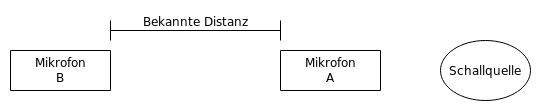
\includegraphics[width=0.9\textwidth]{images/plausibilitaetscheck.png}
        \caption{Versuchsaufbau}
        \label{img:blockschaltbild_plausibilitaetscheck}
\end{figure}

Die beiden Mikrofone sind an einem Oszilloskop angeschlossen. Es werden die \si{AUDIO} und $GATE$ Ausgänge untersucht. Wenn die Schallquelle einen Ton aussendet (durch Klatschen oder ähnliches), passiert es zuerst das Mikrofon A und mit einer Verzögerung Mikrofon B. Mithilfe des bekannten Abstandes der beiden Mikrofone wird untersucht ob das Ergebnis auf dem Oszilloskop mit dem Abstand der Mikrofone übereinstimmt. In der folgenden Abbildung \ref{img:plausibilitaetscheck_oszi} sind vier verschiedene Signale abgebildet. Dabei entspricht Signal \textit{gelb} dem \si{GATE} Ausgang von Mikrofon A und \textit{grün} dem \si{AUDIO} Ausgang. Signal \textit{violett} und \textit{blau} entsprechen dem \si{GATE} und \si{AUDIO} Ausgang von dem zweiten Mikrofon.

\begin{figure}[H]
        \centering
        \hspace*{-1.9cm}
        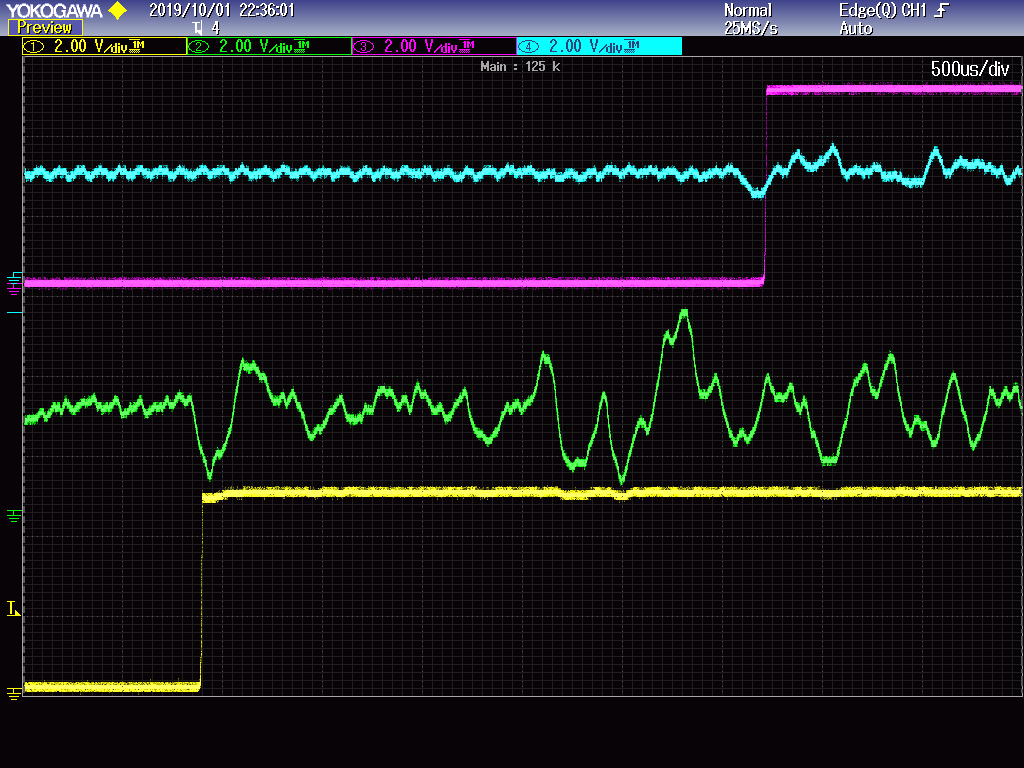
\includegraphics[width=1.2\textwidth]{images/plausibilitaetscheck_oszi.png}
        \caption{Verzögerung der Schallausbreitung}
        \label{img:plausibilitaetscheck_oszi}
\end{figure}

Es ist deutlich erkennbar, dass eine Verzögerung vorhanden ist. Die beiden \si{GATE} Ausgänge liegen ungefähr $2863 \; \mu s$ auseinander. Mit einer Ausbreitungsgeschwindigkeit von $0.034 \; \frac{cm}{\mu s}$ entspricht das ungefähr $97,342 \; cm$. Der gemessene Abstand ist $100 \; cm$. Diese Auswertung zeigt, dass die Verzögerung nur minimal mit dem gemessenen Abstand abweicht. Weiterhin sind die Mirkofone schnell genug in der Erkennung von Schall, welches für eine Positionsbestimmung unerlässlich ist.

\subsubsection{Messung auf einem Board}

Nachdem wir nun wissen, dass das Mikrofon den Anforderungen entspricht, widmen wir uns zunächst einer Zeitmessung auf einem Board. Dabei besitzt das \board \platz Board ein Mikrofon und den Lautsprecher. Es wird untersucht, wie sich eventuelle Ungenauigkeiten bei verschiedenen Entfernungen verhält. Es wurden Messungen mit den Entferungen $50 \; cm$, $100 \; cm$, $200 \; cm$, $300 \; cm$ und $400 \; cm$ gemacht. Die Entfernung kann mit der Gleichung \ref{eq:Entfernung_berechnen} berechnet werden. Die Ausbreitungsgeschwindigkeit von Schall in Luft bei Raumtemperatur entspricht $0.034 \frac{cm}{\mu s}$.
\begin{equation}\label{eq:Entfernung_berechnen}
d \; [cm] = (Empfangszeit - Sendezeit)\;[\mu s]\quad\cdot 0.034 [\frac{cm}{\mu s}]
\end{equation}

Die folgenden Abbildungen (\ref{img:figure_50cm} - \ref{img:figure_400cm}) zeigen jeweils das Messergebnis und ein Histogramm graphisch und den dazugehörigen Mittelwert.

\begin{figure}[H]
	\hspace*{-3.5cm}
    \subfigure[Messwerte bei einer Entfernung von $50 \; cm$]
    {
    	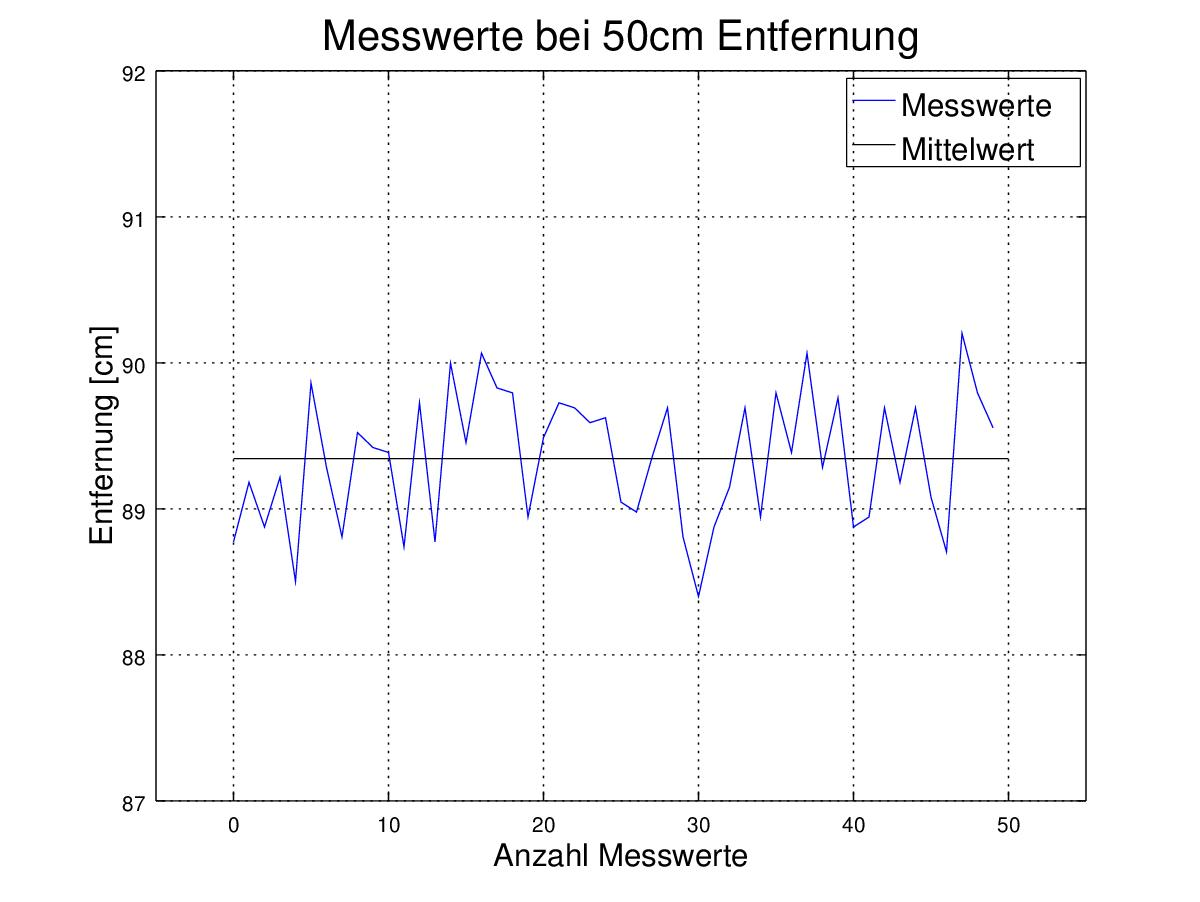
\includegraphics[width=0.7\textwidth]{images/50cm_figure.jpg}
    }
    \subfigure[Histogramm der Messwerte]
    {
    	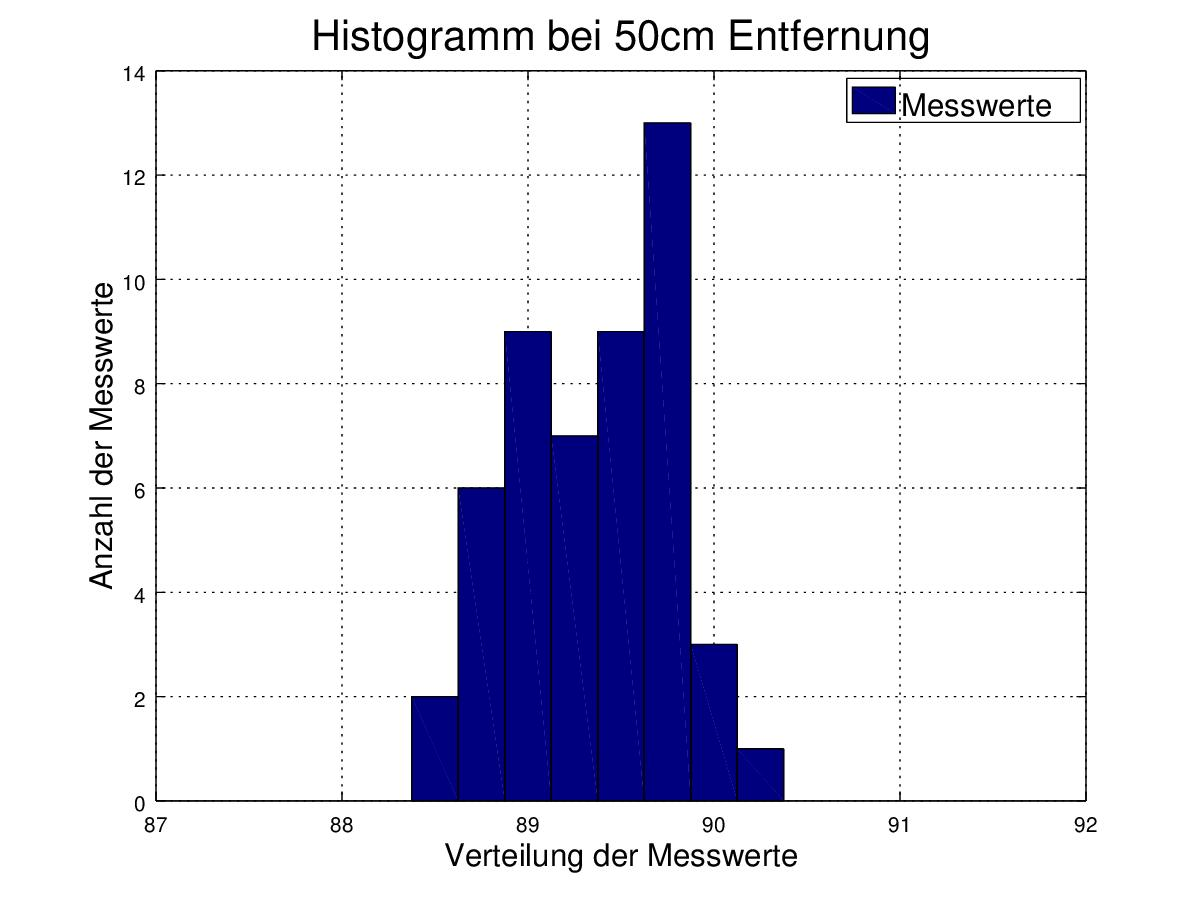
\includegraphics[width=0.7\textwidth]{images/50cm_histogramm.jpg}
    }
	\caption{Messwerte und Verteilung}
	\label{img:figure_50cm}
\end{figure}

\begin{figure}[H]
	\hspace*{-3.5cm}
    \subfigure[Messwerte bei einer Entfernung von $100 \; cm$]
    {
    	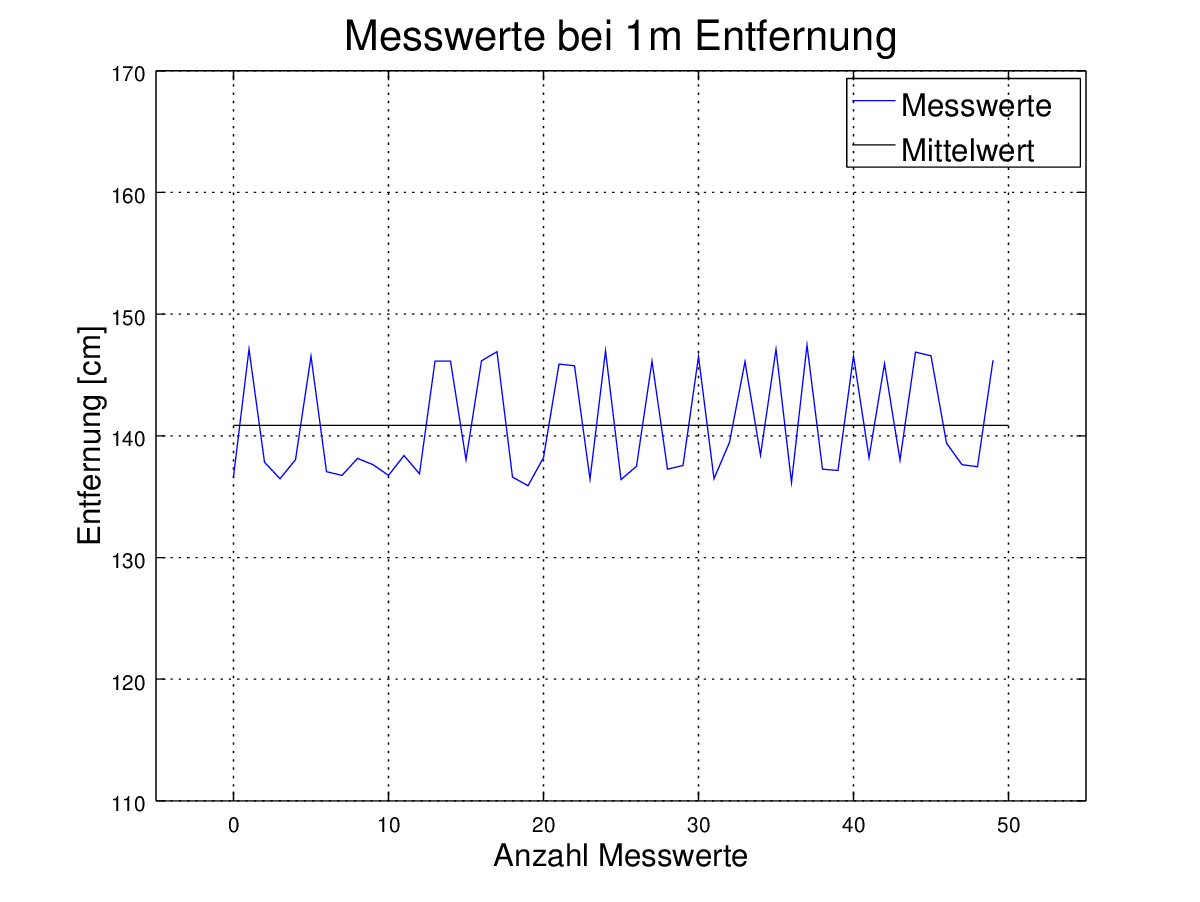
\includegraphics[width=0.7\textwidth]{images/1m_figure.png}
    }
    \subfigure[Histogramm der Messwerte]
    {
    	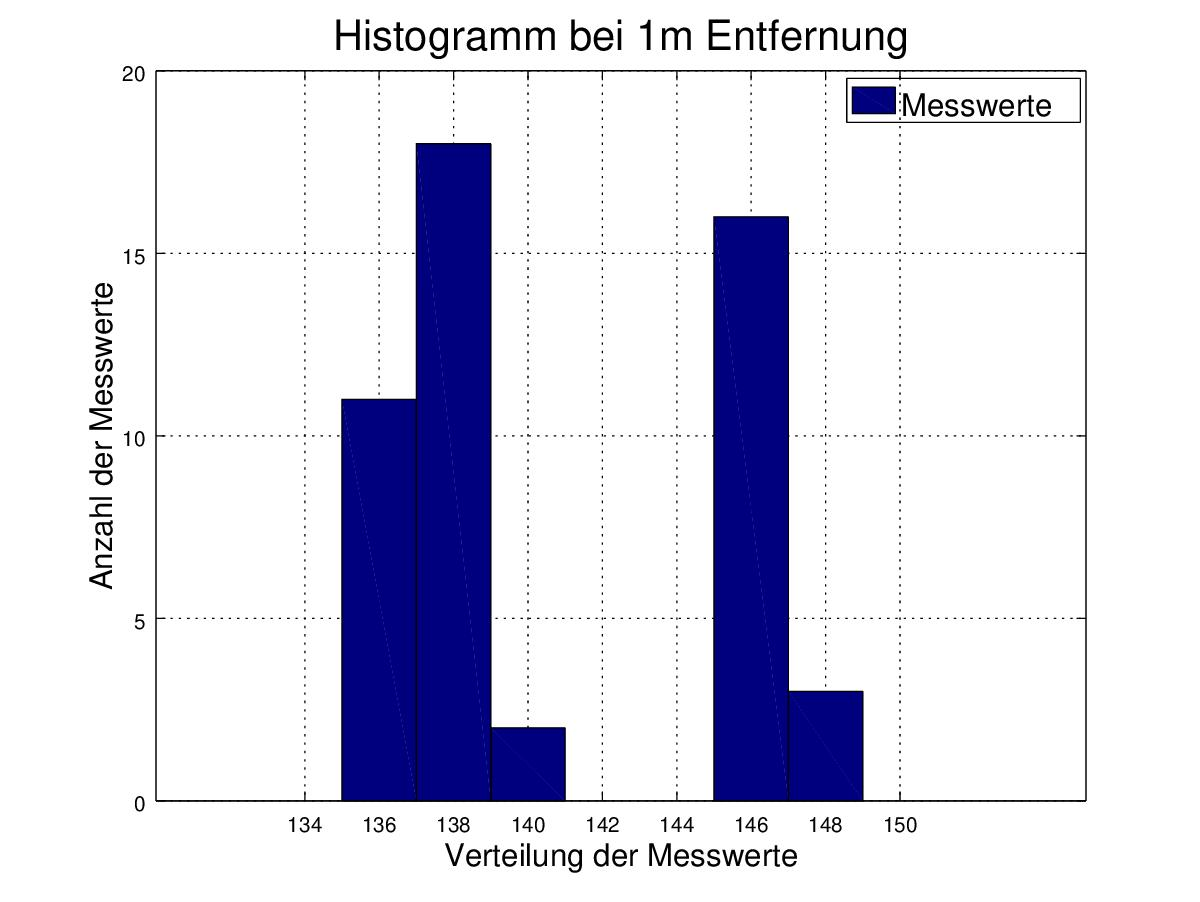
\includegraphics[width=0.7\textwidth]{images/1m_histogramm.jpg}
    }
	\caption{Messwerte und Verteilung}
	\label{img:figure_100cm}
\end{figure}

\begin{figure}[H]
	\hspace*{-3.5cm}
    \subfigure[Messwerte bei einer Entfernung von $200 \; cm$]
    {
    	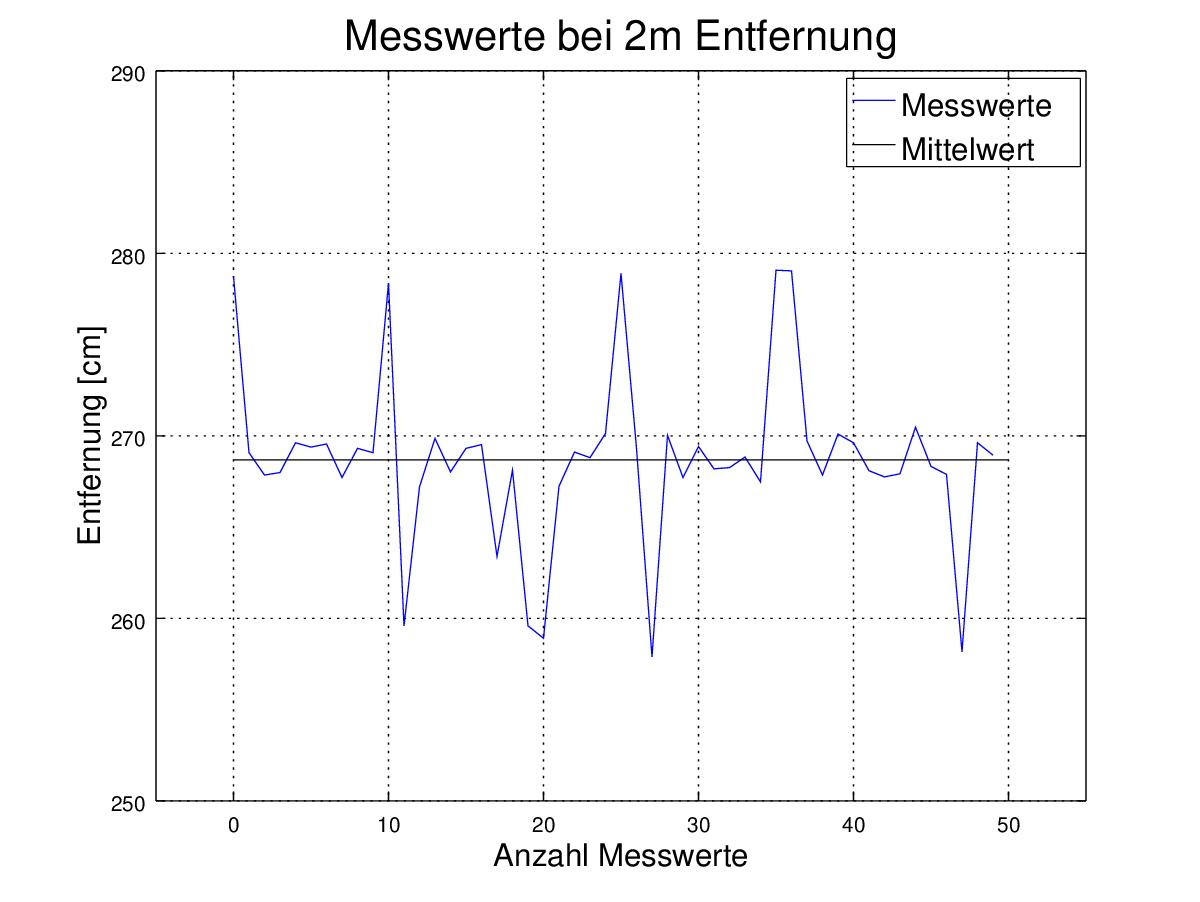
\includegraphics[width=0.7\textwidth]{images/2m_figure.jpg}
    }
    \subfigure[Histogramm der Messwerte]
    {
    	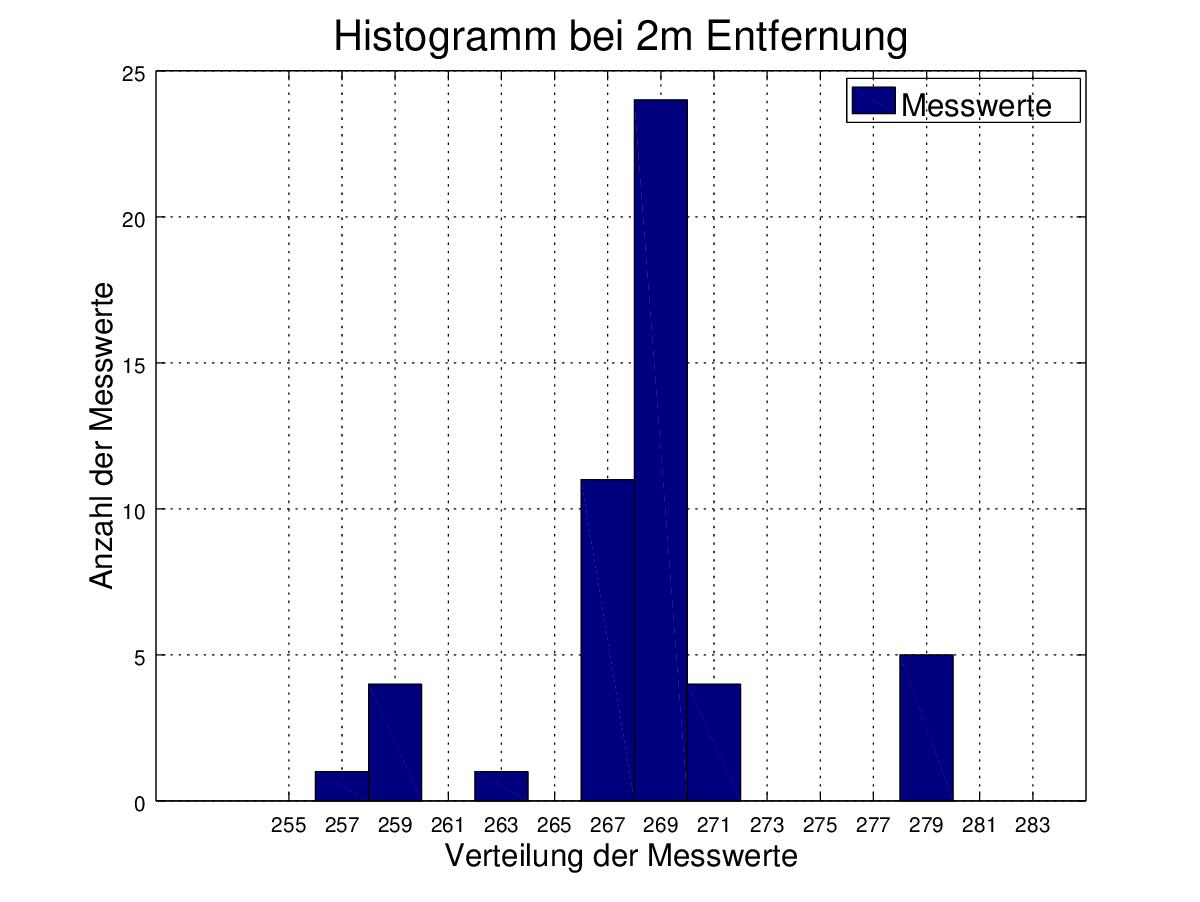
\includegraphics[width=0.7\textwidth]{images/2m_histogramm.jpg}
    }
	\caption{Messwerte und Verteilung}
	\label{img:figure_200cm}
\end{figure}

\begin{figure}[H]
	\hspace*{-3.5cm}
    \subfigure[Messwerte bei einer Entfernung von $300 \; cm$]
    {
    	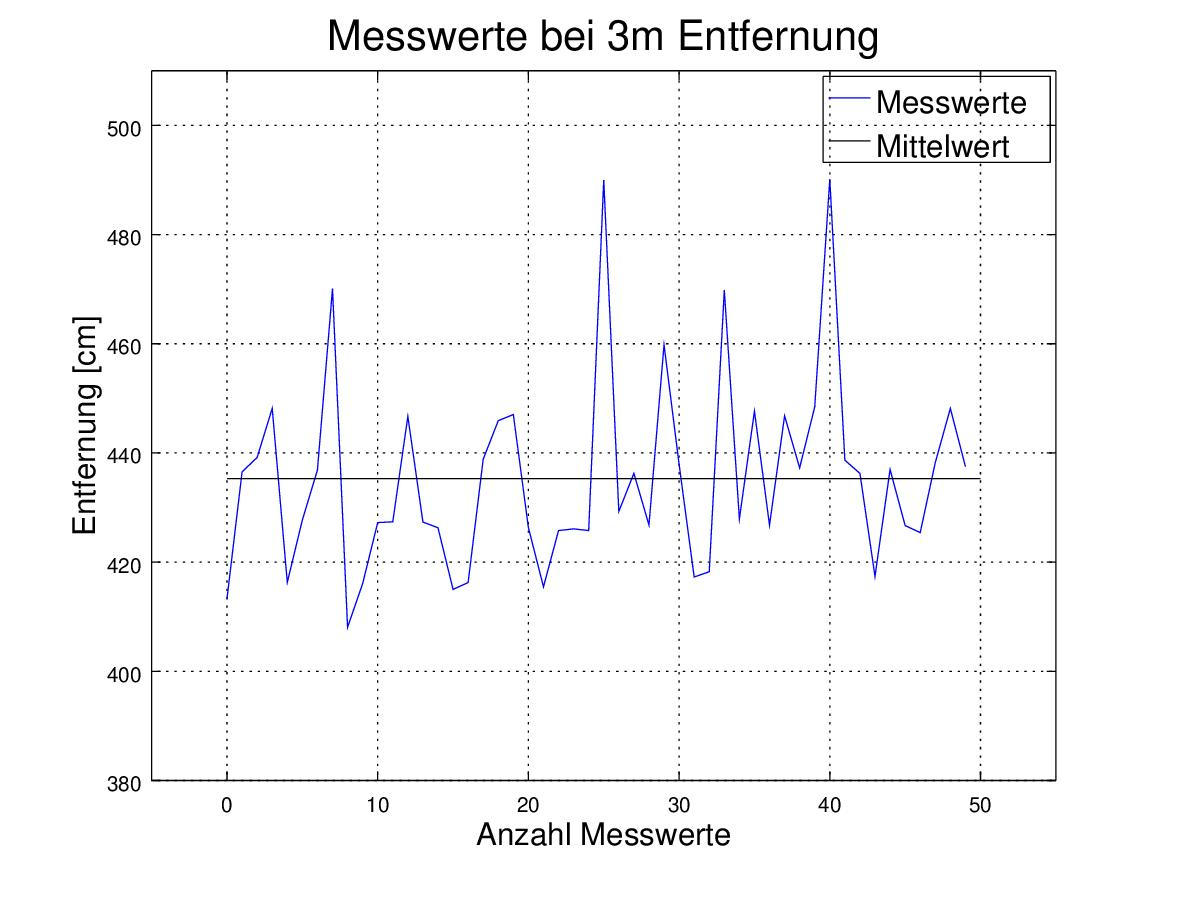
\includegraphics[width=0.7\textwidth]{images/3m_figure.jpg}
    }
    \subfigure[Histogramm der Messwerte]
    {
    	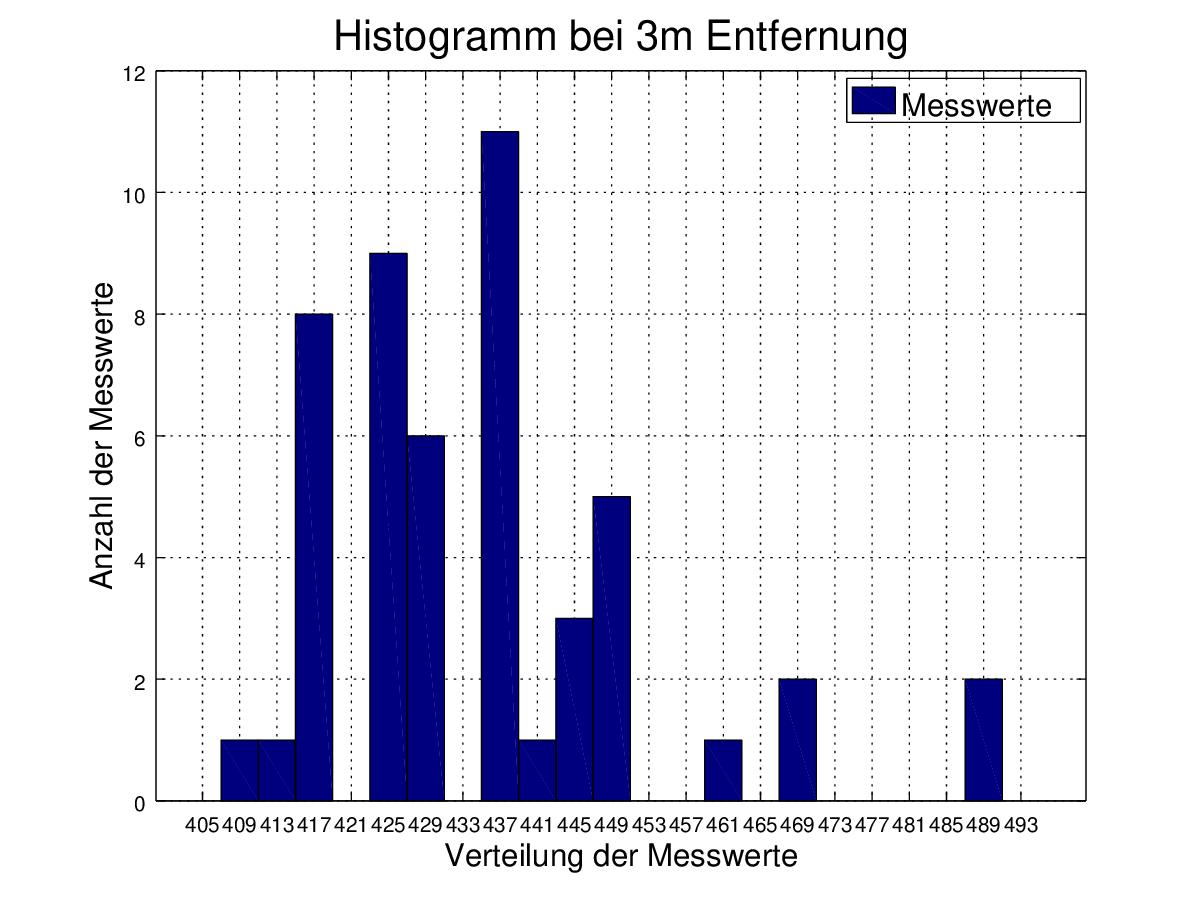
\includegraphics[width=0.7\textwidth]{images/3m_histogramm.jpg}
    }
	\caption{Messwerte und Verteilung}
	\label{img:figure_300cm}
\end{figure}

\begin{figure}[H]
	\hspace*{-3.5cm}
    \subfigure[Messwerte bei einer Entfernung von $400 \; cm$]
    {
    	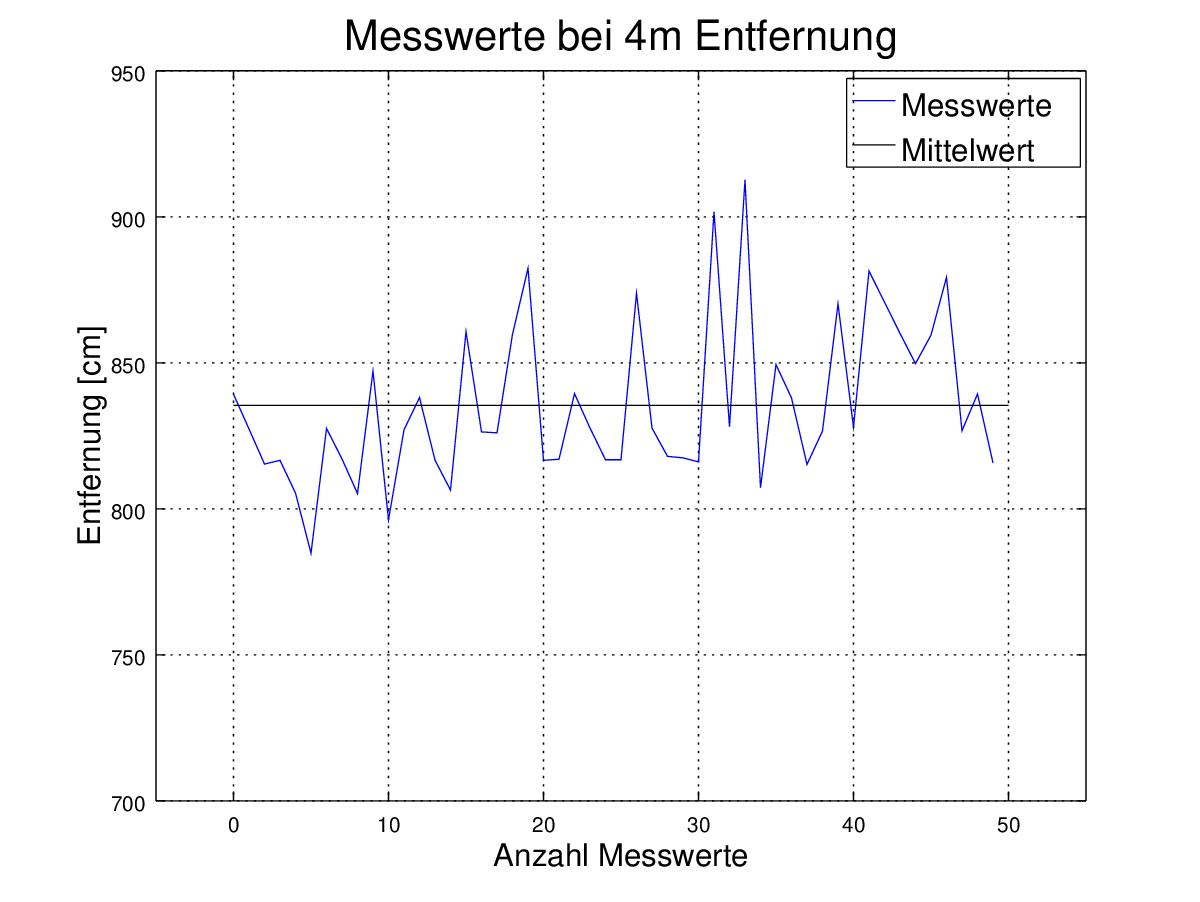
\includegraphics[width=0.7\textwidth]{images/4m_figure.jpg}
    }
    \subfigure[Histogramm der Messwerte]
    {
    	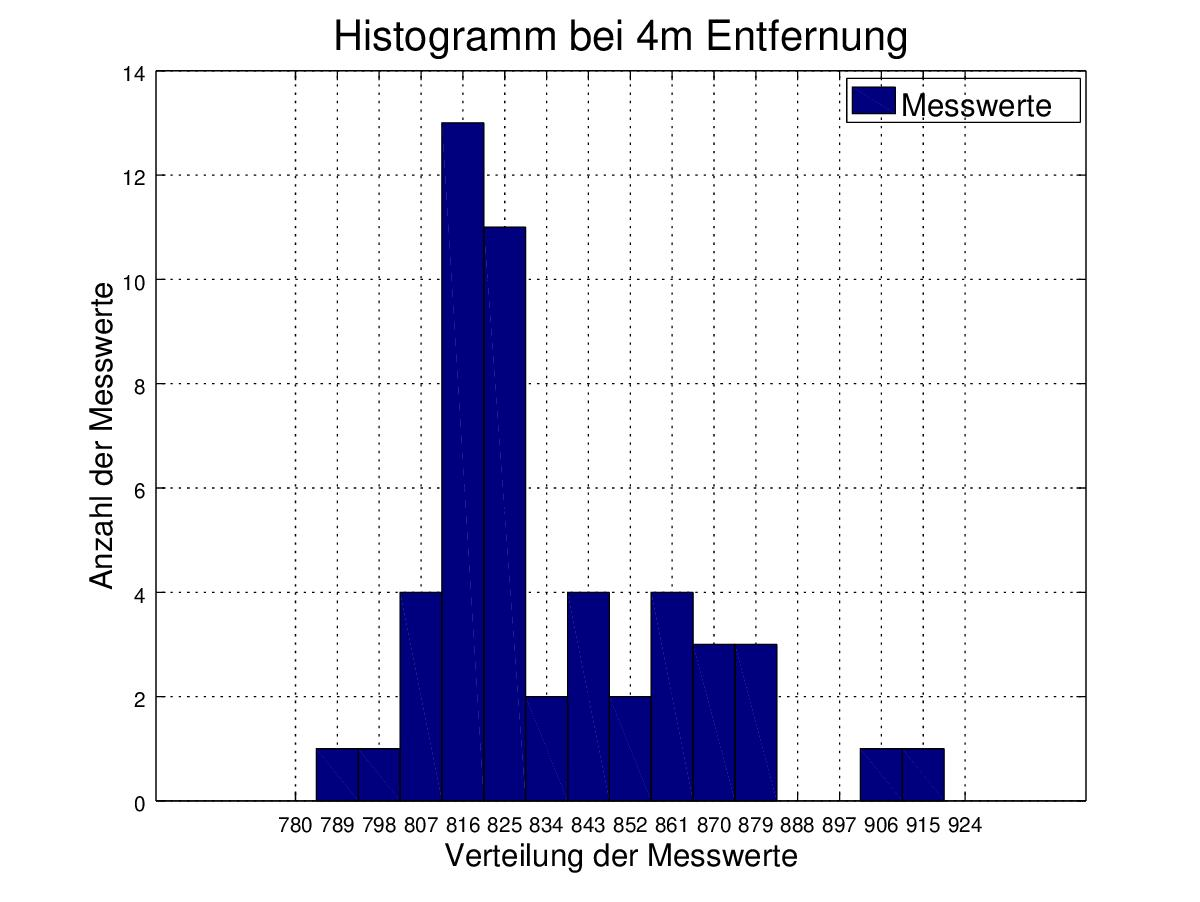
\includegraphics[width=0.7\textwidth]{images/4m_histogramm.jpg}
    }
	\caption{Messwerte und Verteilung}
	\label{img:figure_400cm}
\end{figure}

Zu erkennen ist, dass die Abweichungen mit steigender Distanz zunimmt. Weiterhin kann aus den Histogrammen entnommen werden, dass keine Normalverteilung vorliegt, oder andere Verteilungen vorliegen. Da außerdem keine Muster zu erkennen sind, wirken diese Distanzmessungen willkürlich. Aufgrund der schlechten Ergebnisse, wird noch eine Messung mit zwei Mikrofonen gemacht zusammen mit dem \board .

====================================================

\subsubsection{Zeitsynchronisation}
Bevor die Zeitsynchronisation in die Software eingefügt werden kann, wird geprüft welche Genauigkeit die Zeitsynchronisation erreicht. Dabei werden zwei \board \platz nebeneinander aufgebaut. Es werden insgesamt hundert Zeitsynchronisation nacheinander durchgeführt. Danach werden die Ergebnisse graphisch aufbereitet und ausgewertet. Es wird nur auf die Variable $t_{prop}$ eingegangen, da diese die Differenz zwischen Slave und Master beinhaltet. 
\begin{figure}[H]
        \centering
        \hspace*{-1.7cm}
        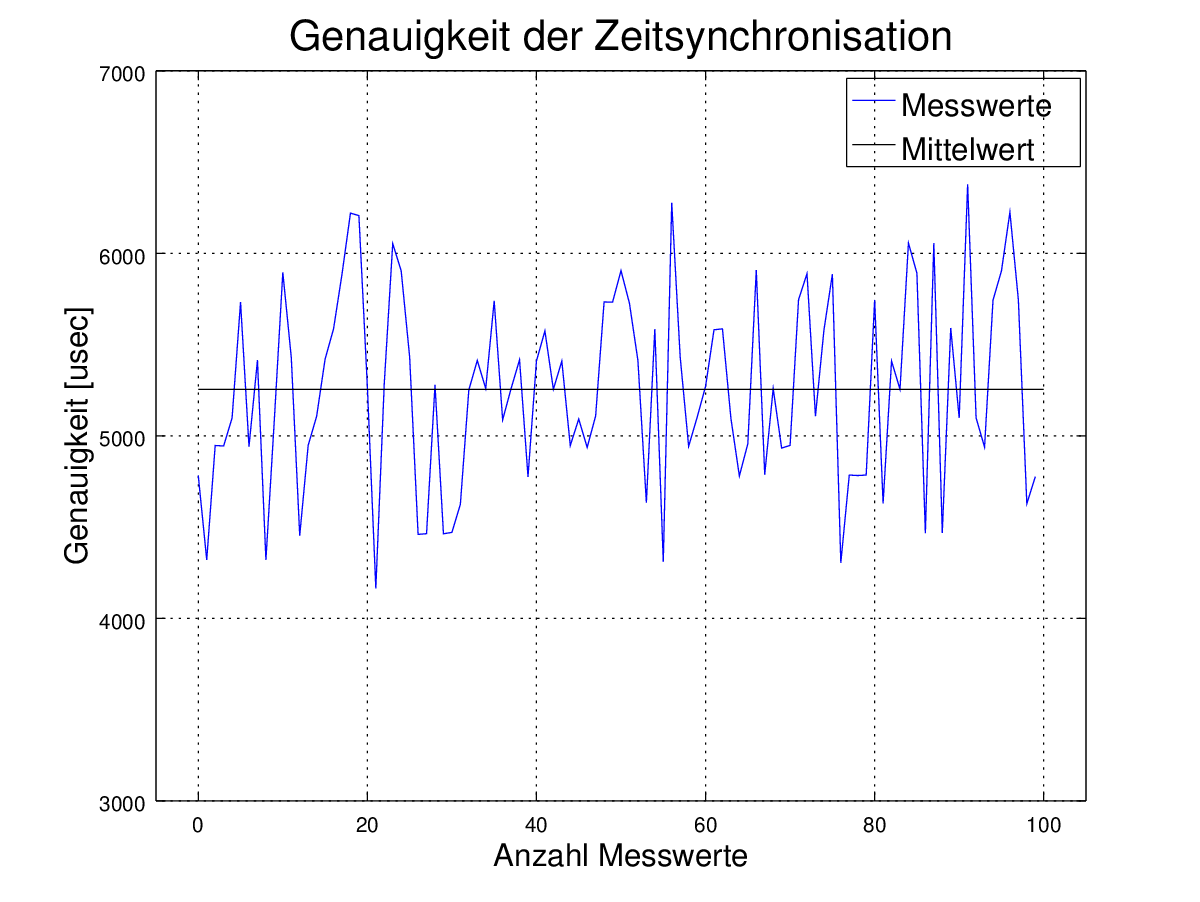
\includegraphics[width=1.2\textwidth]{images/zeit_sync_t_prop_figure.png}
        \caption{Messwerte von $t_{prop}$ bei hundert Messungen}
        \label{img:zeit_sync_t_prop_figure}
\end{figure}
Die obige Abbildung \ref{img:zeit_sync_t_prop_figure} zeigt erreichte Zeitsynchronisation. Da die Zeitsynchronisation sich im Millisekundenbereich bewegt, bedeutet das für die die Positionsbestimmung eine durchschnittliche Abweichung von $178,6394 \;cm$. Das Ergebnis kommt durch die folgende Formel \ref{img:zeit_sync_t_prop_figure} zustande.

\begin{equation}\label{eq:durchschnittsabweichung_t_prop}
5254,1 \;[\mu s] \cdot 0,034 \; [\frac{cm}{\mu s}] = 178,6394 \;[cm]
\end{equation}

Da eine solche Abweichung für eine Zentimetergenaue Positionsbestimmung nicht vertretbar ist, wird für den Start der Messung ein \funkempfaenger \platz verwendet.

============================================

Hier muss noch mehr text zu dem Billigen Funkempfänger rein 434 Mhz ....
\\
============================================

Modul A:




Modul B:


Modul C:

hier gibs keine


Modul D:



Modul E: 1m:

\begin{table}[H]
\begin{tabular}{|c|c|c|c|}
\hline
\multicolumn{4}{|c|}{\textbf{1m Entfernung}}                                                                         \\ \hline
\textbf{Oszilloskop {[}us{]}} & \textbf{Software {[}us{]}} & \textbf{Differenz {[}us{]}} & \textbf{Distanz {[}cm{]}} \\ \hline
4590                          & 4731                       & 141                         & 4,79                      \\ \hline
4630                          & 4784                       & 154                         & 5,23                      \\ \hline
4600                          & 4776                       & 176                         & 5,98                      \\ \hline
4720                          & 4886                       & 166                         & 5,64                      \\ \hline
4600                          & 4766                       & 166                         & 5,64                      \\ \hline
4600                          & 4752                       & 152                         & 5,16                      \\ \hline
4600                          & 4739                       & 139                         & 4,72                      \\ \hline
4580                          & 4753                       & 173                         & 5,88                      \\ \hline
4580                          & 4762                       & 182                         & 6,18                      \\ \hline
4580                          & 4710                       & 130                         & 4,42                      \\ \hline
\multicolumn{4}{|c|}{\textbf{Durchschnitt}}                                                                          \\ \hline
4608                          & 4765                       & 176,10                      & 5,36                      \\ \hline
\end{tabular}
\end{table}

2m:
\begin{table}[H]
\begin{tabular}{|c|c|c|c|}
\hline
\multicolumn{4}{|c|}{\textbf{2m Entfernung}}                                                                         \\ \hline
\textbf{Oszilloskop {[}us{]}} & \textbf{Software {[}us{]}} & \textbf{Differenz {[}us{]}} & \textbf{Distanz {[}cm{]}} \\ \hline
15000                         & 14960                      & 40                          & 1,36                      \\ \hline
48600                         & 48423                      & 177                         & 6,01                      \\ \hline
13900                         & 13940                      & 40                          & 1,36                      \\ \hline
14900                         & 14924                      & 24                          & 0,81                      \\ \hline
21500                         & 21508                      & 8                           & 0,27                      \\ \hline
12700                         & 12710                      & 10                          & 0,34                      \\ \hline
13800                         & 13973                      & 173                         & 5,88                      \\ \hline
13800                         & 14013                      & 213                         & 7,24                      \\ \hline
12000                         & 11999                      & 1                           & 0,03                      \\ \hline
13600                         & 13647                      & 47                          & 1,59                      \\ \hline
\multicolumn{4}{|c|}{\textbf{Durchschnitt}}                                                                          \\ \hline
17980,00                      & 18009,70                   & 73,30                       & 2,49                      \\ \hline
\end{tabular}
\end{table}

3m:
\begin{table}[H]
\begin{tabular}{|c|c|c|c|}
\hline
\multicolumn{4}{|c|}{\textbf{3m Entfernung}}                                                                         \\ \hline
\textbf{Oszilloskop {[}us{]}} & \textbf{Software {[}us{]}} & \textbf{Differenz {[}us{]}} & \textbf{Distanz {[}cm{]}} \\ \hline
21900                         & 21906                      & 6                           & 0,20                      \\ \hline
23900                         & 23908                      & 8                           & 0,27                      \\ \hline
19000                         & 19019                      & 19                          & 0,64                      \\ \hline
23100                         & 23224                      & 124                         & 4,21                      \\ \hline
19700                         & 19665                      & 35                          & 1,19                      \\ \hline
21300                         & 21310                      & 10                          & 0,34                      \\ \hline
20742                         & 20700                      & 42                          & 1,42                      \\ \hline
23200                         & 23278                      & 78                          & 2,65                      \\ \hline
18100                         & 18090                      & 10                          & 0,34                      \\ \hline
20100                         & 20014                      & 86                          & 2,92                      \\ \hline
\multicolumn{4}{|c|}{\textbf{Durchschnitt}}                                                                          \\ \hline
21104,20                      & 22919,20                   & 41,80                       & 1,42                      \\ \hline
\end{tabular}
\end{table}



F:
\begin{table}[H]
\begin{tabular}{|c|}
\hline
\textbf{Messwert {[}us{]}} \\ \hline
77,20                      \\ \hline
71,80                      \\ \hline
84,20                      \\ \hline
69,60                      \\ \hline
95,20                      \\ \hline
70,40                      \\ \hline
90,80                      \\ \hline
68,60                      \\ \hline
93,60                      \\ \hline
83,00                      \\ \hline
\textbf{Durchschnitt}      \\ \hline
70,34                      \\ \hline
\end{tabular}
\end{table}



G 1m:
\begin{table}[H]
\begin{tabular}{|c|c|c|}
\hline
\multicolumn{3}{|c|}{\textbf{1m Entfernung}}                                         \\ \hline
\textbf{Messwert {[}us{]}} & \textbf{Differenz {[}us{]}} & \textbf{Distanz {[}cm{]}} \\ \hline
5,14                       & 2,19                        & 74,76                     \\ \hline
5,14                       & 2,19                        & 74,76                     \\ \hline
4,87                       & 1,92                        & 65,58                     \\ \hline
4,87                       & 1,92                        & 65,58                     \\ \hline
5,15                       & 2,20                        & 75,10                     \\ \hline
4,88                       & 1,93                        & 65,92                     \\ \hline
4,87                       & 1,92                        & 65,58                     \\ \hline
4,90                       & 1,95                        & 66,60                     \\ \hline
4,89                       & 1,94                        & 66,26                     \\ \hline
4,90                       & 1,95                        & 66,60                     \\ \hline
\multicolumn{3}{|c|}{\textbf{Durchschnitt}}                                          \\ \hline
4,96                       & 2,01                        & 68,67                     \\ \hline
\end{tabular}
\end{table}








2m:
\begin{table}[H]
\begin{tabular}{|c|c|c|}
\hline
\multicolumn{3}{|c|}{\textbf{2m Entfernung}}                                         \\ \hline
\textbf{Messwert {[}us{]}} & \textbf{Differenz {[}us{]}} & \textbf{Distanz {[}cm{]}} \\ \hline
11,38                      & 5,49                        & 186,92                    \\ \hline
11,08                      & 5,19                        & 176,72                    \\ \hline
11,66                      & 5,77                        & 196,44                    \\ \hline
11,72                      & 5,83                        & 198,48                    \\ \hline
12,00                      & 6,11                        & 208,00                    \\ \hline
11,12                      & 5,23                        & 178,00                    \\ \hline
11,48                      & 5,59                        & 190,32                    \\ \hline
11,14                      & 5,25                        & 178,76                    \\ \hline
11,72                      & 5,83                        & 198,48                    \\ \hline
11,44                      & 5,55                        & 188,96                    \\ \hline
\multicolumn{3}{|c|}{\textbf{Durchschnitt}}                                          \\ \hline
11,47                      & 5,59                        & 190,10                    \\ \hline
\end{tabular}
\end{table}


3m:
\begin{table}[H]
\begin{tabular}{|c|c|c|}
\hline
\multicolumn{3}{|c|}{\textbf{3m Entfernung}}                                         \\ \hline
\textbf{Messwert {[}us{]}} & \textbf{Differenz {[}us{]}} & \textbf{Distanz {[}cm{]}} \\ \hline
23,95                      & 15,12                       & 514,30                    \\ \hline
35,70                      & 26,87                       & 913,80                    \\ \hline
31,75                      & 22,92                       & 779,50                    \\ \hline
24,25                      & 15,42                       & 524,50                    \\ \hline
30,75                      & 21,92                       & 745,50                    \\ \hline
22,30                      & 13,47                       & 458,20                    \\ \hline
22,30                      & 13,47                       & 458,20                    \\ \hline
34,00                      & 25,17                       & 856,00                    \\ \hline
23,60                      & 14,77                       & 502,40                    \\ \hline
26,15                      & 17,32                       & 589,10                    \\ \hline
\multicolumn{3}{|c|}{\textbf{Durchschnitt}}                                          \\ \hline
27,47                      & 18,65                       & 634,15                    \\ \hline
\end{tabular}
\end{table}



\subsubsection{Genauigkeit}
Die Genauigkeit spielt bei der Positionsbestimmung eine entscheidene Rolle. Je größer die Ungenauigkeit, desto größer wird der Bereich, indem sich der Zielknoten befinden kann. Dadurch das jede Kommunikation Verlustbehaftet ist, ist eine geringe Ungenauigkeit nicht zu vermeiden. Eine PingPong Kommunikation von Zielknoten und Accesspoint, hat eine durschschnittliche Verzögerung von $9.4492\; ms$. Dabei wurde hundertmal ein \si{PING}-Kommando ausgesendet welches mit einem \si{PONG} beantwortet wurde und der Mittelwert gebildet. Diese Verzögerung kann allerdings mit der Zeitsynchronisation ausgeglichen werden. Aus der Verzögerung aus den Abbildungen \ref{img:figure_50_cm} - \ref{img:figure_400_cm} kann keine Genauigkeit im Zentimeterbereich erreicht werden, da kein Muster zu erkennen ist. Diese Ungenauigkeit kann nur mit veränderter Hardware verbessert werden. Aufgrund der schlechten Genauigkeit wird diese Arbeit nicht über das Labor hinaus eingesetzt.  


\subsubsection{Positionsbestimmung}
Um nun die Positionsbestimmung durchzuführen, verhält sich die Software nach dem folgenden Programmablaufplan \ref{img:PAP}. Zuerst wird der Zeitunterschied ausgeglichen der zwischen den Accesspoints (Slaves) und dem Zielknoten (Master) besteht. Dafür wird das bereits beschriebene PTP Protokoll verwendet. Erst nachdem die Zeitsynchronisation erfolgreich ist, werden Messungen vorgenommen. Dabei spricht der Master einzeln die Slaves an. Der Master gibt zu einem bestimmten Zeitpunkt vor, wann der enstprechende Slave den Lautsprecher für $40000 \; \mu s$ einschaltet. Über das Mikrofon beim Master wird der Ton empfangen und es wird sofort die Systemzeit bestimmt. Über die Differenz vom Aussenden und Empfangen kann die Distanz berechnet werden.
\begin{figure}[H]
        \centering
        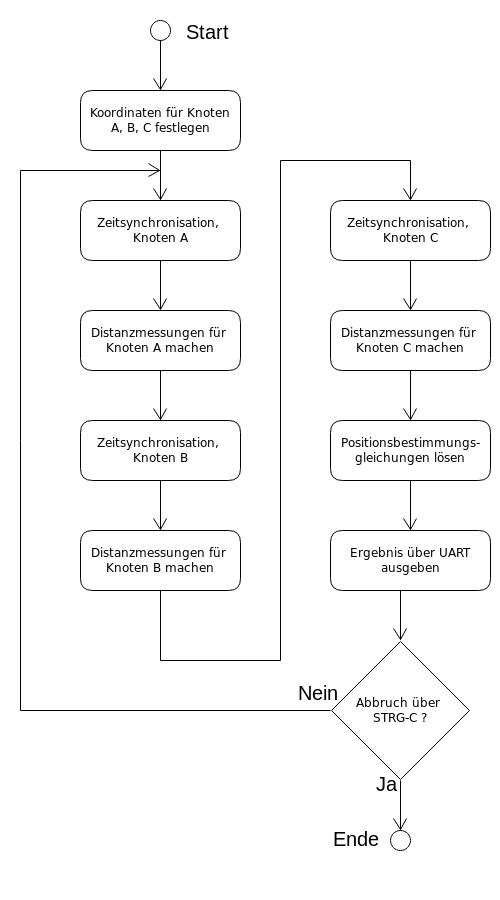
\includegraphics[width=0.8\textwidth]{images/PAP.png}
        \caption{Programmablaufplan der Software}
        \label{img:PAP}
\end{figure}

Dieses Vorgehen wird für alle drei Slaves wiederholt. Zusammen mit den Koordinaten der Slaves ergeben sich auf einer Ebene drei Kreise, die sich schneiden. Der Schnittpunkt der Kreise ist foglich die Position des Masters. Über die Tastenkombination STRG-C kann die Positionsbestimmung abgebrochen werden. Geschieht dies nicht, wird die Messung für alle drei Slaves wiederholt. Somit kann der Master sich auf der Ebene bewegen und bekommt seine Postion angezeigt. Es muss bedacht werden, dass durch den Jitter des Frequenzgebers die Systemzeit der Slaves mit der Zeit divergieren, d.h, wartet man entsprechend lange, ist die Systemzeit der Slaves nicht mehr übereinstimmend mit dem Master. Deswegen muss regelmäßig eine Zeitsynchronisation erfolgen. Da diese Arbeit unter Laborbedinungen durchgeführt wird, gibt es nur eine Zeitsynchronisation.

\subsection{Evaluierung}
Für die Evaluierung der Positionsbestimmung wird ein Prototyp aufgebaut. Dieser findet unter Laborbedinungen statt. Dabei kommen folgende Komponenten zum Einsatz.

\begin{itemize}
\item 4x \board \platz mit Lautsprecher als Accesspoint
\item 1x \board \platz mit \microphone \platz als Zielknoten
\end{itemize}

Abbildung \ref{img:prototyp} zeigt den Aufbau aus der Vogelperspektive. Dabei ist der Zielknoten nur examplarisch in der Mitte plaziert. Bei der Versuchsdurchführung

\begin{figure}[H]
        \centering
        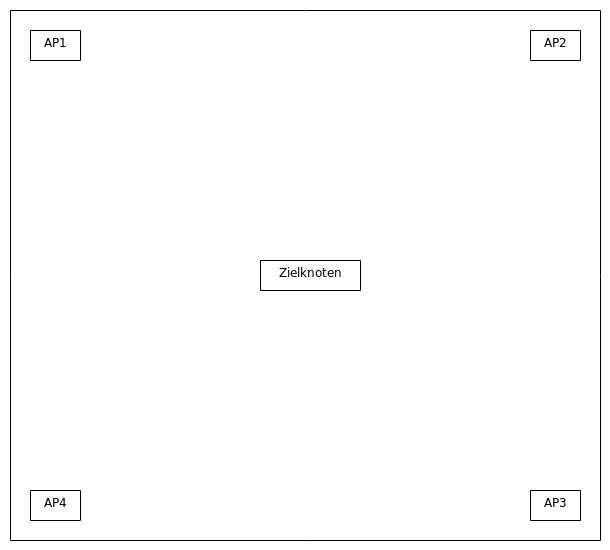
\includegraphics[width=0.7\textwidth]{images/prototyp.png}
        \caption{Aufbau aus der Vogelperspektive}
        \label{img:prototyp}
\end{figure}

